%page style
\pagestyle{fancy}
\vspace*{40 pt}

\subsection{Tela alarmes}

Esta tela exibe os alarmes que ocorreram na máquina. Os alarmes são exibidos em ordem de ocorrência, sendo o mais recente exibido no topo da lista.
A tela possui um botão para resetar a lista de alarmes, ver log de alarmes e overview fornecendo uma ampla consiencia operacional de uma forma simples e intuitiva.
Ao pressionar o botão ver log de alarmes é possível visualizar todos os alarmes que ocorreram na máquina em uma lista ordenada por data e hora.
Para acessar esta tela, basta clicar no botão "Alarmes" em qualquer tela.

%inserir a imagem da tela
\begin{figure}[h]
  \centering
  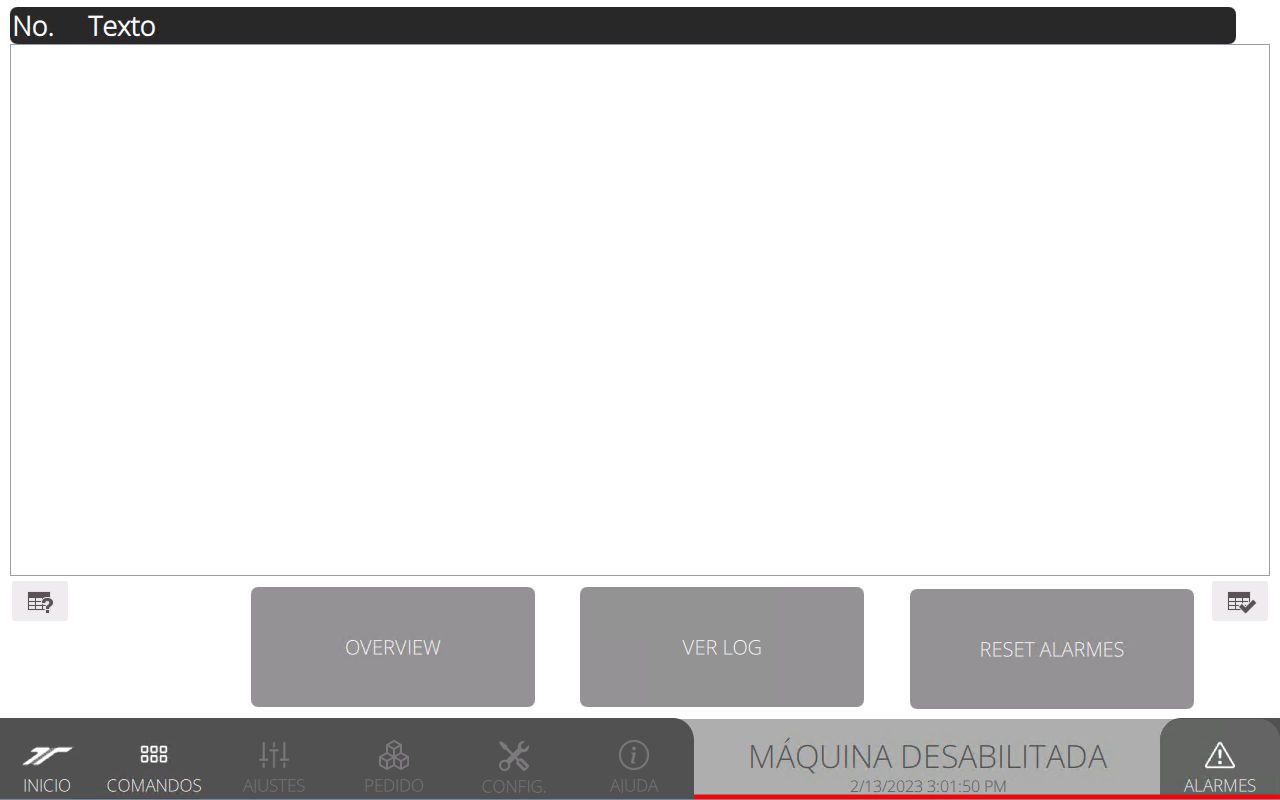
\includegraphics[width=480 px,height=300 px]{src/imagesICV/13-alarmsScreen/e-Tela-Principal.png}
\end{figure}

\newpage
\pagestyle{fancy}
\vspace*{40 pt}

\subsubsection{\small{Overview Geral}}

Esta tela pode ser acessada clicando no botão "Overview" na tela de alarmes. Ela exibe uma representação gráfica da máquina e dos alarmes que ocorreram. 
Os alarmes são representados por ícones coloridos, sendo que a cor alaranjada significa que o alarme está ativo e a cor cinza o contrário. Algums icones representam
a posição do alarme na máquina e outros representam apenas que existe este tipo de alarme na unidade porém sua posição não significa que o alarme está naquele lugar. Para
retornar a tela de alarmes, basta clicar em qualquer lugar da tela em que não haja um ícone.

\begin{figure}[h]
    \centering
    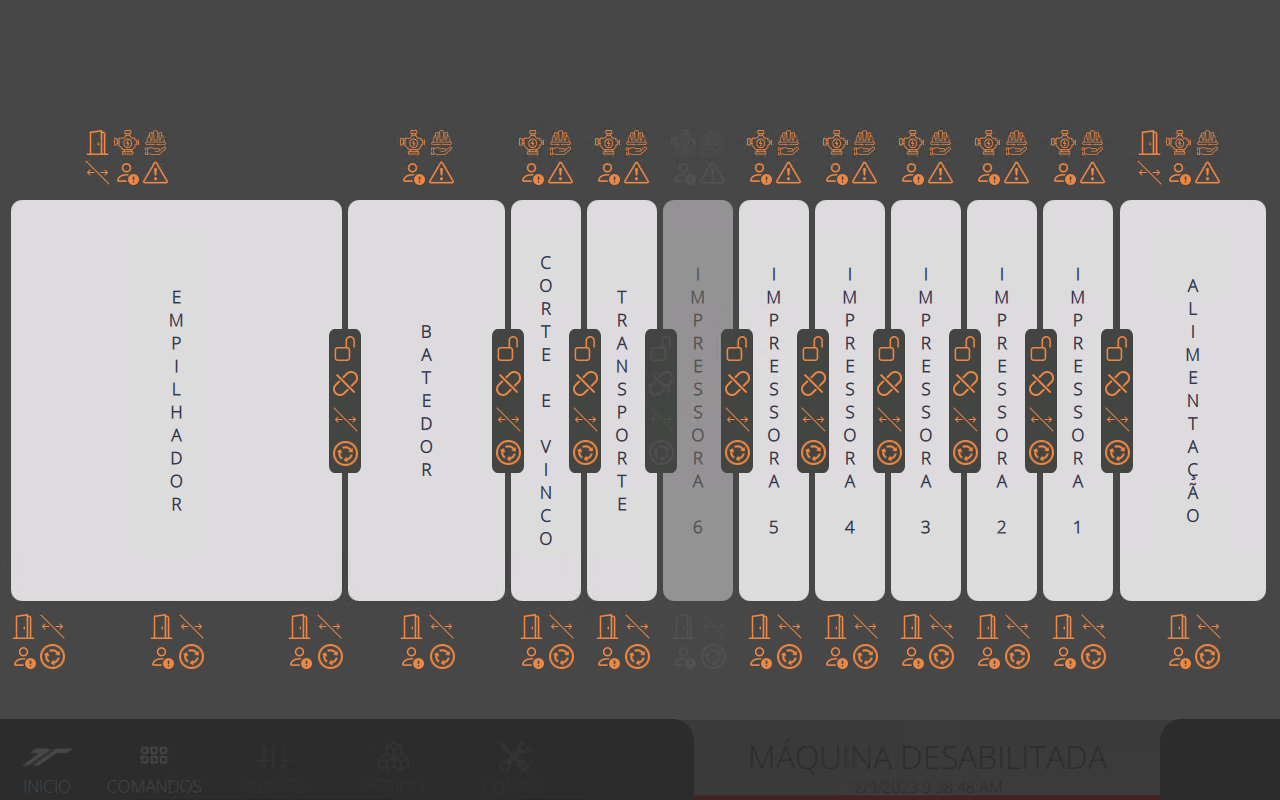
\includegraphics[width=384 px,height=240 px]{src/imagesICV/13-alarmsScreen/telaOverview.png}
  \end{figure}

O significado de cada ícone pode ser visto na lista abaixo:

\newlist {alarmIcons2}{itemize}{1}
  \setlist [alarmIcons2]{label={}, nosep, before=\vspace{10pt}, after=\vspace{10pt}}

\begin{alarmIcons}

\item[\ding{\dingNumber}] 
\includegraphics[height=1em]{src/imagesICV/13-alarmsScreen/overview/disconnect-orange.png} Unidade desacoplada.
\item[\ding{\dingNumber}] 
\includegraphics[height=1em]{src/imagesICV/13-alarmsScreen/overview/don't-move-orange.png} Bloqueio do equipamento ativo, sinaliza a posição da chave.
\item[\ding{\dingNumber}] 
\includegraphics[height=1em]{src/imagesICV/13-alarmsScreen/overview/door-open-orange.png} Porta aberta no equipamento, sinaliza a posição da porta.
\item[\ding{\dingNumber}] 
\includegraphics[height=1em]{src/imagesICV/13-alarmsScreen/overview/emergency-stop-orange.png} Botão de emergência pressionado, sinaliza a posição do botão.
\item[\ding{\dingNumber}] 
\includegraphics[height=1em]{src/imagesICV/13-alarmsScreen/overview/engine-orange.png} Alarme em um motor na unidade.
\item[\ding{\dingNumber}] 
\includegraphics[height=1em]{src/imagesICV/13-alarmsScreen/overview/exclamation-triangle-orange.png} Alarme ativo na unidade.
\item[\ding{\dingNumber}] 
\includegraphics[height=1em]{src/imagesICV/13-alarmsScreen/overview/helmet-orange.png} STO ativo na unidade.
\item[\ding{\dingNumber}] 
\includegraphics[height=1em]{src/imagesICV/13-alarmsScreen/overview/unlock-orange.png} Alarme unidade destravada.
\item[\ding{\dingNumber}] 
\includegraphics[height=1em]{src/imagesICV/13-alarmsScreen/overview/person-exclamation-orange.png} Indica um acesso interno na unidade. 
Indica qual unidade e em qual lado ocorreu o acesso.


\end{alarmIcons}

\newpage
\pagestyle{fancy}
\vspace*{40 pt}

\subsubsection{\small{Overview de uma unidade}}

Esta tela pode ser acessada clicando no nome da unidade na tela Overview. Ela exibe uma representação gráfica dos servos na unidade e dos alarmes presentes neles.
A lógica dos icones é semelhante a tela "Overview". Além da representação gráfica, é possível visualizar os cartões de IO da unidade podendo identificar quais entradas
e saídas estão sendo utilizadas, no caso de entradas safety é mostrado qual entrada está com problemas. Para retornar a tela de Overview, 
basta clicar em qualquer lugar da tela em que não haja um ícone.

\begin{figure}[h]
    \centering
    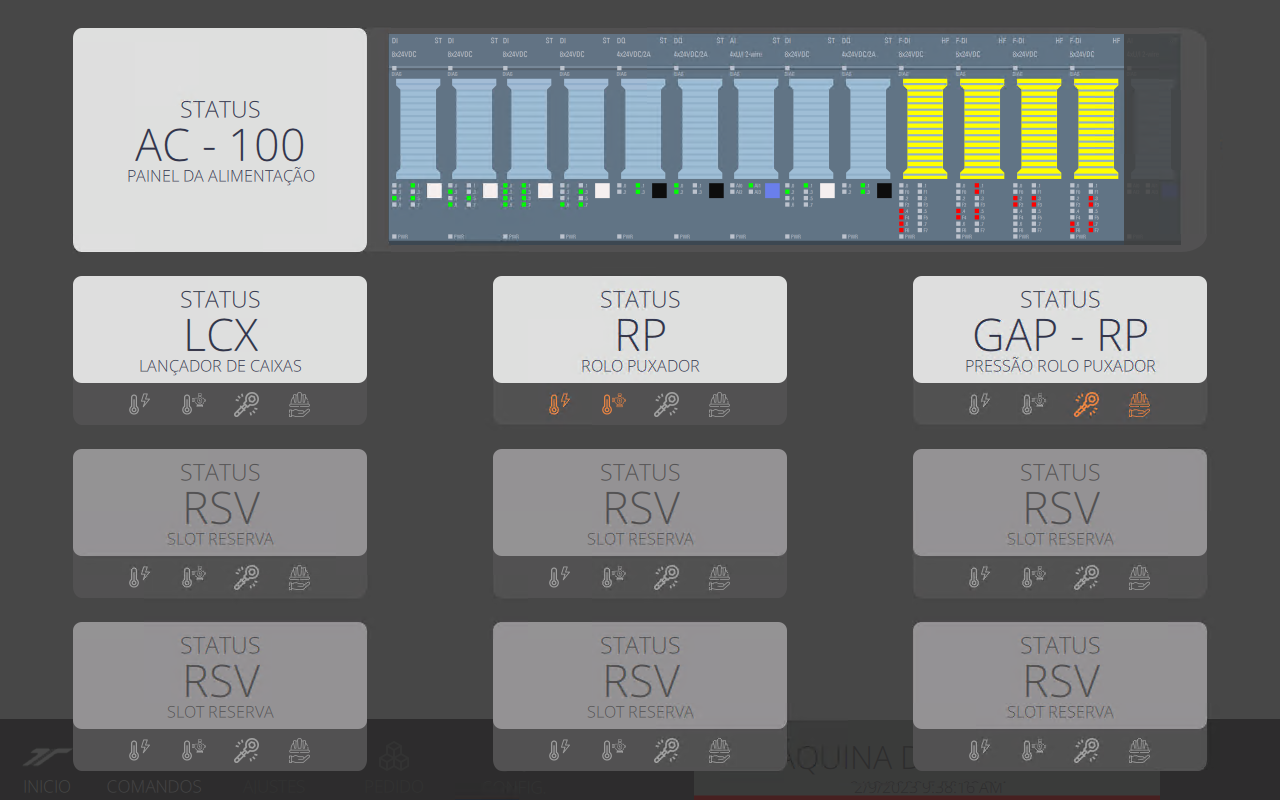
\includegraphics[width=384 px,height=240 px]{src/imagesICV/13-alarmsScreen/overviewUnidades.png}
  \end{figure}

O significado de cada ícone pode ser visto na lista abaixo:

\newlist {unityAlarmIcons2}{itemize}{1}
  \setlist [unityAlarmIcons2]{label={}, nosep, before=\vspace{10pt}, after=\vspace{10pt}}

\begin{unityAlarmIcons}

\item[\ding{\dingNumber}] 
\includegraphics[height=1em]{src/imagesICV/13-alarmsScreen/overview/drive-overtemperature-light-orange.png} Alarme de sobreaquecimento do drive.
\item[\ding{\dingNumber}] 
\includegraphics[height=1em]{src/imagesICV/13-alarmsScreen/overview/motor-overtemperature-orange.png} Alarme de sobreaquecimento do motor.
\item[\ding{\dingNumber}] 
\includegraphics[height=1em]{src/imagesICV/13-alarmsScreen/overview/torque-wrench-orange.png} Alarme de torque excedido.
\item[\ding{\dingNumber}] 
\includegraphics[height=1em]{src/imagesICV/13-alarmsScreen/overview/helmet-orange.png} STO ativo no servo.

\end{unityAlarmIcons}










